\ifdefined\USERMANUAL
  \newcommand{\doctype}{PODRECZNIK UŻYTKOWNIKA}
\else
  \newcommand{\doctype}{KARTY REFERENCYJNE}
\fi

\maketitlepage{TAIPO}{Rozszerzenie MIDI}{TAIPO_SILVER_cutout_small_2}{\doctype}
\newpage
\tableofcontents

\newpage
\part{Przegląd}
\newpage
\section{Przegląd}\label{section:installation}
\subsection{Przegląd}
\paragraph*{}
\textbf{TAIPO} MIDI Extender dla The Centre umożliwia podłączenie The Centre
do zewnętrznego sprzętu (w tym komputera) za pomocą standardowego kabla MIDI TRS typu B.
\subsection{Co jest w pudełku}
\paragraph*{}\textbf{TAIPO} jest dostarczany ze standardowymi akcesoriami. Wewnątrz pudełka znajdziesz:
\begin{enumerate}
  \item Moduł Eurorack \textbf{TAIPO}
  \item Standardowy kabel zasilający Eurorack (10-pin do 16-pin)
  \item Kabel połączeniowy MIDI-EX do połączenia z \textbf{THE CENTRE}
\end{enumerate}

\newpage
\part{Instalacja}
\newpage
\section{Instalacja}
\subsection{Kroki instalacji}
\paragraph*{}
Instalacja TAIPO przebiega zgodnie z krokami instalacji dowolnego modułu Eurorack w obudowie właściciela.

\begin{figure}[h]
  \centering
  \includegraphics[height=0.5\linewidth]{taipo_the_centre_cable_install.jpg}
  \includegraphics[height=0.5\linewidth]{taipo_cable_install.jpg}
  \caption{Instalacja kabla po obu stronach}
  \label{fig:midsinglenote}
\end{figure}

\subsection{Ważne uwagi dotyczące instalacji}
\paragraph*{}
Proszę zwrócić uwagę na kolejność kolorów po obu stronach. Kolejność kolorów po stronie The Centre od góry powinna być \textbf{CZARNY, CZERWONY, ŻÓŁTY, ZIELONY}, a po stronie TAIPO odwrotnie: \textbf{ZIELONY, ŻÓŁTY, CZERWONY, CZARNY}
\newline$\blacksquare$ WAŻNE: Po stronie The Centre podłącz do złącza MIDI-EX, jak pokazano na powyższym obrazku. Drugie złącze służy do podłączenia wyjścia MIDI The Centre do TWINS.

\newpage
\part{MIDI}
\newpage
\section{Typy kabli MIDI}
\subsection{Typ kabla TAIPO}
\paragraph*{}
TAIPO używa kabla MIDI TRS typu B Zobacz: \underline{\nameref{section:cabletypeb}}
\subsection{O sygnale MIDI}
\paragraph*{}
Sygnał MIDI jest wysyłany kablem MIDI przy użyciu standardowego protokołu RS232, jednak z 
nestandardową prędkością 31250 bodów (bitów na sekundę). Połączenie elektryczne MIDI jest 
kierunkowe, co oznacza, że wewnętrzne połączenie pinów w kablu ma znaczenie, ponieważ prąd
płynie w jednym kierunku. Chociaż nie stanowi to problemu w przypadku standardowych kabli MIDI typu DIN, 
stało się to problematyczne w przypadku kabli opartych na jack 3,5 mm (TRS), ponieważ producenci zaczęli je okablowywać

inaczej, ponieważ nie zdefiniowano żadnego standardu. Na podstawie tych okablowań pojawiło się kilka

standardów. 
\newline$\blacksquare$ Różne standardy TRS nie są wymienne i nie są kompatybilne. 
Aby podłączyć urządzenia o różnych standardach TRS, należy użyć odpowiedniego kabla.
\subsection{Złącze DIN}
Standardowy kabel MIDI wykorzystujący 5-pinowe złącze DIN
\subsection{Typy złączy TRS}
\subsubsection{Złącze typu A}
TRS Typ A definiuje \textbf{TIP} gniazda 3,5 mm jako \textit{\textbf{źródło}}, a \textbf{RING} jako \textit{\textbf{ujście}}
\newline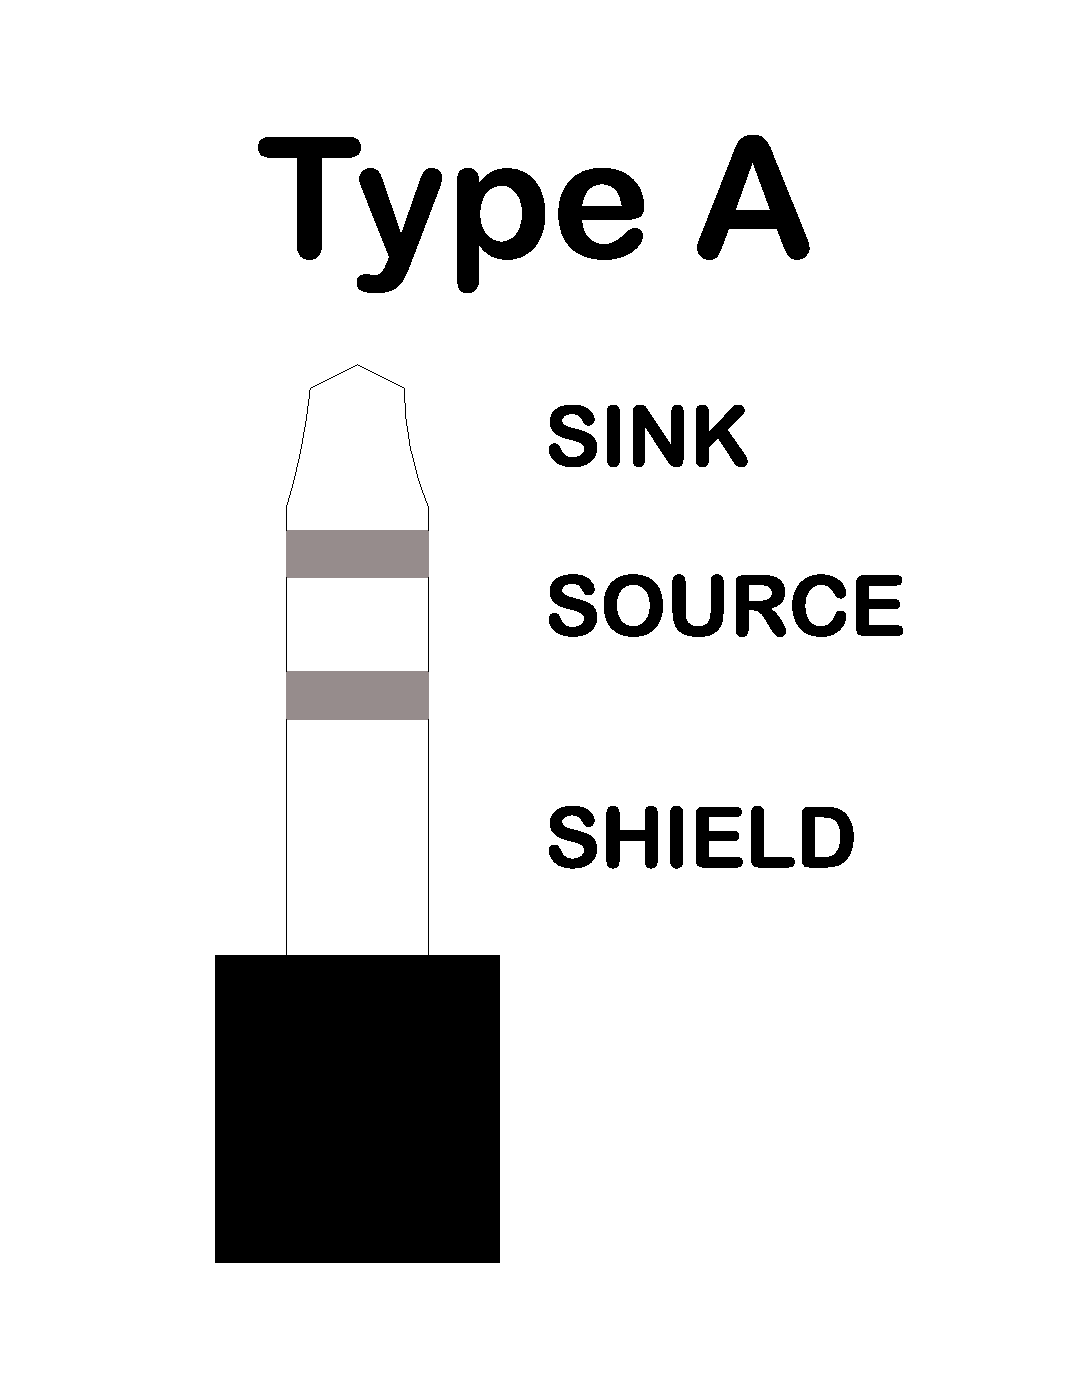
\includegraphics[height=0.3\linewidth]{midi_trs_type_a.eps}
\newline$\bigstar$ Marki używające typu A: Korg, Akai
\subsubsection{Złącze typu B}\label{section:cabletypeb}
TRS Typ B definiuje \textbf{TIP} gniazda 3,5 mm jako \textit{\textbf{ujście}}, a \textbf{RING} jako \textit{\textbf{źródło}}
\newline$\blacksquare$ Typ B jest bardziej popularny na scenie modularnej Eurorack
\newline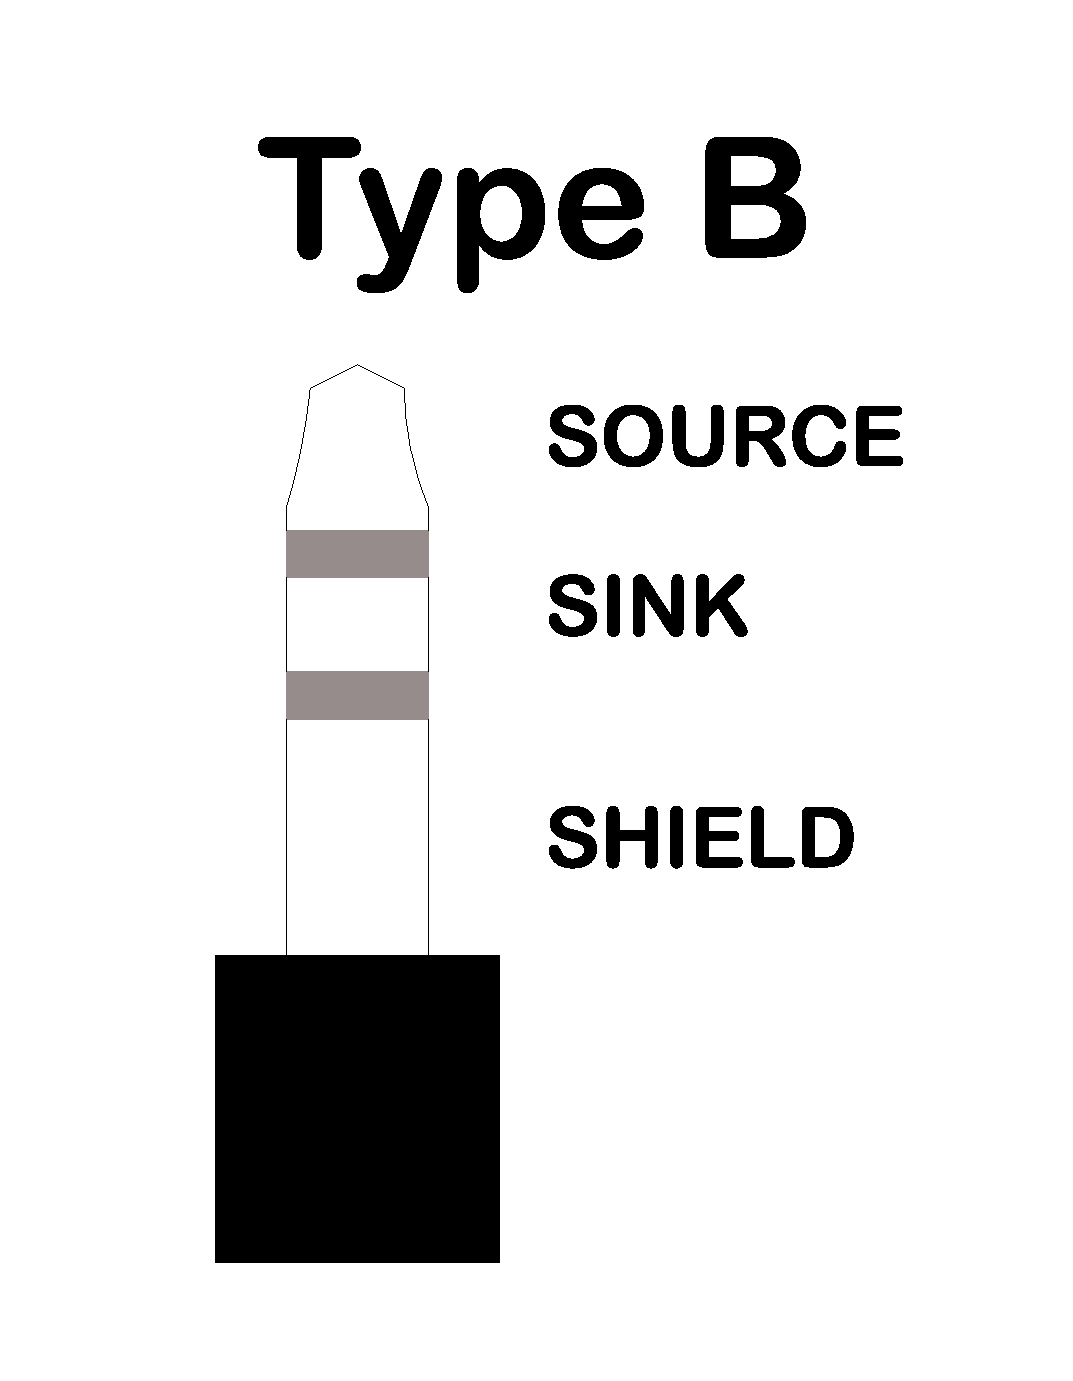
\includegraphics[height=0.3\linewidth]{midi_trs_type_b.eps}
\newline$\bigstar$ Marki używające typu B: Arturia, Novation, 1010
